% -*- mode: TeX -*-
% -*- coding: utf-8 -*-

% \documentclass[10pt, conference]{IEEEtran}
% \usepackage[utf8]{inputenc}
%
% \usepackage{amssymb}
%
% \usepackage[pdftex]{graphicx}
%\graphicspath{{./images/}}
%\DeclareGraphicsExtensions{.pdf,.jpeg,.png}
%
% \usepackage[tight,footnotesize]{subfigure} % old version
% \usepackage{todonotes}
%
% %\usepackage[caption=false]{caption} % keep ieee style fix for subfig package
% %\usepackage[font=footnotesize]{subfig}
%
%
% \usepackage{url}
%
%
% % correct bad hyphenation here
% \hyphenation{op-tical net-works semi-conduc-tor log-in}
%
%
% %*** ALIGNMENT PACKAGES ***
%
% \usepackage{array}
% \usepackage{mdwmath}
% \usepackage{mdwtab} % WARNING: screws up \multicolumn usage in tables!

%\usepackage{fixltx2e}
%\usepackage{stfloats}


%*** colors ***
% \usepackage{xcolor,colortbl}
 \definecolor{colorRowHeader}{rgb}{0.976471,0.976471,0.976471}
 \definecolor{colorSubLine}{rgb}{0.5,0.5,0.5}

%*** tables ***
% \usepackage{multirow}
% \usepackage{booktabs}
%\usepackage{arydshln} % dashed lines in tables. % vertical by : or ;{1pt/1pt} in the header. % horizontal by \cdashline{2-3}[1pt/1pt] 
% e.\,g.\ \\ \arrayrulecolor{colorSubLine} \cdashline{2-3}[1pt/1pt] \arrayrulecolor{black}

%*** code ***
%\usepackage{listings}
%\lstset{language=Pascal}
% \usepackage{algorithm}
% \usepackage{algorithmicx} % loaded by algpseudocode
% \usepackage{algpseudocode}

%*** definitions ***
% \newcommand{\etal}{ et\,al. }
% \newcommand{\eg}{e.\,g.,\ } % note the trailing comma (recommended by http://grammar.quickanddirtytips.com/ie-eg-oh-my.aspx )
% \newcommand{\ie}{i.\,e.,\ }
\newcommand{\seclabel}[1]{\label{section:passwords-peer-to-peer:#1}}
\newcommand{\subseclabel}[1]{\label{subsection:passwords-peer-to-peer:#1}}
\newcommand{\subsubseclabel}[1]{\label{subsubsection:passwords-peer-to-peer:#1}}
\newcommand{\figlabel}[1]{\label{figure:passwords-peer-to-peer:#1}}
\newcommand{\algolabel}[1]{\label{algorithm:passwords-peer-to-peer:#1}}
\newcommand{\tablabel}[1]{\label{table:passwords-peer-to-peer:#1}}
\newcommand{\secref}[1]{Section~\ref{section:passwords-peer-to-peer:#1}}
\newcommand{\subsecref}[1]{Section~\ref{subsection:passwords-peer-to-peer:#1}}
\newcommand{\subsubsecref}[1]{Section~\ref{subsubsection:passwords-peer-to-peer:#1}}
\newcommand{\figref}[1]{Figure~\ref{figure:passwords-peer-to-peer:#1}}
\newcommand{\algoref}[1]{Algorithm~\ref{algorithm:passwords-peer-to-peer:#1}}
\newcommand{\tabref}[1]{Table~\ref{table:passwords-peer-to-peer:#1}}

% \begin{document}

% \title{Passwords in Peer-to-Peer}

% \author{\IEEEauthorblockN{Gunnar Kreitz, Oleksandr Bodriagov, Benjamin
% Greschbach, Guillermo Rodr\'{i}guez-Cano, and Sonja Buchegger }
% \IEEEauthorblockA{
% KTH Royal Institute of Technology\\ School of Computer Science and
% Communication\\ Stockholm, Sweden \\\{gkreitz, obo, bgre, gurc, buc\}@csc.kth.se}
% }

% author names and affiliations
% use a multiple column layout for up to two different
% affiliations

%\author{\IEEEauthorblockN{TODO}
%\IEEEauthorblockA{
%KTH Royal Institute of Technology\\ School of Computer Science and
%Communication\\ Stockholm, Sweden \\\{TODO\}@csc.kth.se}
%}

% \maketitle
\begin{center}
Gunnar Kreitz, Oleksandr Bodriagov, Benjamin Greschbach,\\
Guillermo Rodr\'{i}guez-Cano, and Sonja Buchegger\\[2em]

KTH Royal Institute of Technology\\
School of Computer Science and Communication\\
Stockholm, Sweden\\
% \{gkreitz, obo, bgre, gurc, buc\}@csc.kth.se
\{\href{gkreitz@csc.kth.se}{gkreitz}, \href{obo@csc.kth.se}{obo}, 
\href{bgre@csc.kth.se}{bgre}, \href{gurc@csc.kth.se}{gurc}, \href{buc@csc.kth.se}{buc}\}@csc.kth.se
\end{center}


\begin{abstract}
One of the differences between typical peer-to-peer (P2P) and client-server
systems is the existence of user accounts. While many P2P applications, like
public file sharing, are anonymous, more complex services such as
decentralized online social networks require user authentication. In these,
the common approach to P2P authentication builds on the possession of
cryptographic keys. A drawback with that approach is usability when users
access the system from multiple devices, an increasingly common scenario.

In this work, we present a scheme to support logins based on users knowing a
username-password pair. We use passwords, as they are the most common
authentication mechanism in services on the Internet today, ensuring strong
user familiarity. In addition to password logins, we also present supporting
protocols to provide functionality related to password logins, such as
resetting a forgotten password via e-mail or security questions. Together,
these allow P2P systems to emulate centralized password logins. The
results of our performance evaluation  indicate that incurred delays
are well within acceptable bounds.
\end{abstract}

\clearpage
\section{Introduction}

Most of the peer-to-peer (P2P) systems deployed today do not authenticate
users. While this is is often acceptable, or even preferable, there are some
problems for which user authentication is a requirement. These include P2P
storage, backup, and online social networks. In such applications, the data
accessible to a client depends on who is using it.

We discuss how to implement a username-password scheme for  authentication
in P2P systems. Our goal is to construct an authentication
component that can be reused across different P2P applications, which we assume 
authenticate via possession of cryptographic keys. Thus, from an API 
perspective, the login system shall allow a user entering a username and a password
to recover a set of cryptographic keys which can then be used by the actual
application. These keys can also be updated as needed
by the application.

The goal from an end-user point of view is to emulate current behavior 
of centralized password-based login mechanisms. More specifically,
we include schemes to remember logins, change passwords, and provide
recovery if a password is forgotten.  We aim to follow best practice in
password authentication, acknowledging that users often re-use passwords
between systems. By remembered logins, we mean that a user can opt to have
a device store information such that it can log in again without storing the
user's password in plain text on the device. 
Similarly, password change requires knowing the old password, and for
password recovery, the user is able to set a new password but does not learn
her previous one.

% Our system builds on a few underlying primitives which are common in many P2P
% systems. To handle user registration, we build upon a global key-value store,
% which can be realized either as a Distributed Hash Table (DHT), or as a
% cloud service. To store information required by our protocols, we assume
% the existence of distributed storage. We assume the storage system
% authenticates via cryptographic keys. Finally, to support password recovery
% via e-mail, we assume there is a mechanism to (uniformly randomly) sample
% peers in the system. This can be solved \eg via a gossiping protocol.

\subsection{Why password authentication?}

There is a rich literature on various approaches to authentication, ranging
from the traditional username-password pair to hardware tokens and
biometry. Of these, the traditional view is that passwords should be replaced
by some better mechanism. However, as argued by Herley and
van~Oorschot~\cite{HerleyO12}, despite significant research efforts into
dislodging passwords, they are still by far the most common authentication
mechanism today. Reasons for their prevalence include simplicity, price, and
very strong user familiarity.

When authentication is required in the P2P setting, it is typically done
via the security-wise stronger mechanism of generating and storing
cryptographic keys on a user's machine. This approach is taken in systems such
as OneSwarm~\cite{IsdalPKA10}, Safebook~\cite{Cutillo09a}, and
Tribler~\cite{AbbasPES09}.  This works well until the user wants to access the service from a second
device. To do so, she would need to transfer the keys, or assume a new
identity. This is an added complexity and user-perceived drawback for P2P
services competing against client-server systems.

One concern is that using passwords may lead to added security risks
for skilled and security-conscious users who can easily copy keys
between devices.  However, nothing prevents such users from choosing
passwords of similar strength as cryptographic keys. Another issue
pertains to remembered logins, where one must consider theft. We
cannot prevent a thief from accessing the user's account, but with our
protocols, the thief cannot change the user's password, and the
legitimate user can always revoke the remembered credentials that are
on the stolen device.

\subsection{Our Contribution}
We develop and describe a suite of protocols for password
authentication in P2P networks: account registration, login,
password change, remembered logins, logout also of a remote device, and password
recovery, following best practices and adapting standardized criteria
from centralized systems to P2P environments, and start a
discussion on usable authentication in P2P systems.

Our password authentication is based on standard
cryptographic techniques and can be used with standard P2P components. As a
first step toward a security analysis, we discuss the security implications of
our protocols. Then, we evaluate the performance of our protocols under various
scenarios.

\subsection{Paper Outline}
We discuss related work in \secref{relatedwork}, give a system
overview in \secref{systemsoverview} and outline our basic scheme for
password-based login in \secref{passwordlogin}. We then describe
password recovery mechanisms as extensions to the basic login
mechanisms in \secref{recovery}. Next, we discuss security in
\secref{security} and report our evaluation results in
\secref{evaluation} before concluding in \secref{conclusions}.

\section{Related Work} \seclabel{relatedwork}

The subject of securely establishing stable identities in P2P systems has been
previously studied, for instance by Aberer, Datta and
Hauswirth~\cite{AbererDH04}. The need for identities mainly arose from
technical concerns, such as handling dynamic IP address assignment, or
avoiding Sybil attacks~\cite{Douceur02}. Authentication of a node is done via
a signature key, automatically generated and stored on the node.

As P2P systems began providing more complex functionality
\cite{IsdalPKA10,Cutillo09a,AbbasPES09,LillibridgeEBBI03}, the need to authenticate
\emph{users}, rather than nodes, arose. It seems that often, authentication
via a signature key has been carried over to this problem. While a solution
of automatic identification of a node is preferable as long as users use a
single device, equating a node with a user fails as users increasingly access
services from multiple devices.

Illustrative is the case of backup systems, where an important use case is to
restore data on a different system from where it was backed up. Here, two
different approaches to authentication have been taken. All approaches build
on encrypting backed up content, and the approaches vary in whether the keys
are randomly derived~\cite{LillibridgeEBBI03}, or derived from a password
\cite{CoxMN02}. In the former case, a user must manually
back the keys up, as these keys are required to restore the backup. The
systems deriving a key from a password are related to our proposed protocol,
and use some related techniques. However, to the best of our knowledge, they
do not consider the additional protocols required surrounding password
authentication, such as remembered logins, and recovering lost passwords.

Some P2P storage systems also use techniques which are related to ours.
For example, the DHT-based systems 
GNUnet and Freenet use keyword strings to derive a public-private key pair
whose private key is used to sign data and the hash of the public key to
identify the data in the storage. Both of these systems use a keyword string
as a seed to a pseudo-random number generator that produces the key pair
\cite{Clarke10,Bennett03}. Knowing only the memorable keyword string the user
can store and retrieve information.

%Authentication via passwords is also used in some peer-assisted
%systems\footnote{By peer-assisted, we mean a centralized system where P2P is
%used for offloading.} systems, such as Spotify and Wuala\footnote{Wuala is no
%longer peer-assisted, here we describe the old system.}. These two systems use
%passwords in different ways. Spotify implements a traditional centralized
%authentication, while Wuala derives a key from the user's password and uses it
%locally to encrypt backed-up files. We note that Wuala does not offer a
%mechanism to recover forgotten passwords~\cite[``I forgot my password, what
%now?'']{WualaFAQ}.

Related to forgotten passwords, recovery of information in a
P2P scenario has been studied by Vu\etal \cite{Vu_Aberer_Buchegger_Datta_2009}
who proposed a combination of threshold-based secret sharing with delegate
selection and encrypting shares with passwords.

Frykholm and Juels~\cite{FrykholmJ01} proposed a password-recovery mechanism
based on security questions very similar to our protocol for the same task.
They offer better, information-theoretic security properties, something
not applicable to our scenario. % \eg security against a computationally unbounded attacker. 
We treat the subject of password change, which is not
applicable to their scenario, although their proposal could be extended to support
password change using our techniques.

\section{System Overview and Assumptions} \seclabel{systemsoverview}

We have designed our system around standard primitives, as
depicted in \figref{systemoverview}.  In particular, our protocols
build on: a DHT~\cite{WehrleGR05,JimenezOK11}, for user lookup; a peer sampling
protocol~\cite{JelasityVGKS07,BortnikovGKKS09} for randomly choosing peers; and a distributed
storage~\cite{BennettGHP02,RheaEGWZK03} for storing data required for our
solution. Both the DHT and distributed storage are P2P protocols, run by the
peers participating in the system. The storage could be implemented as a DHT,
or even be the same as the user lookup DHT. However, we put different
requirements on the user lookup DHT and the distributed storage, as detailed
below.

\begin{figure}
  \centering
  %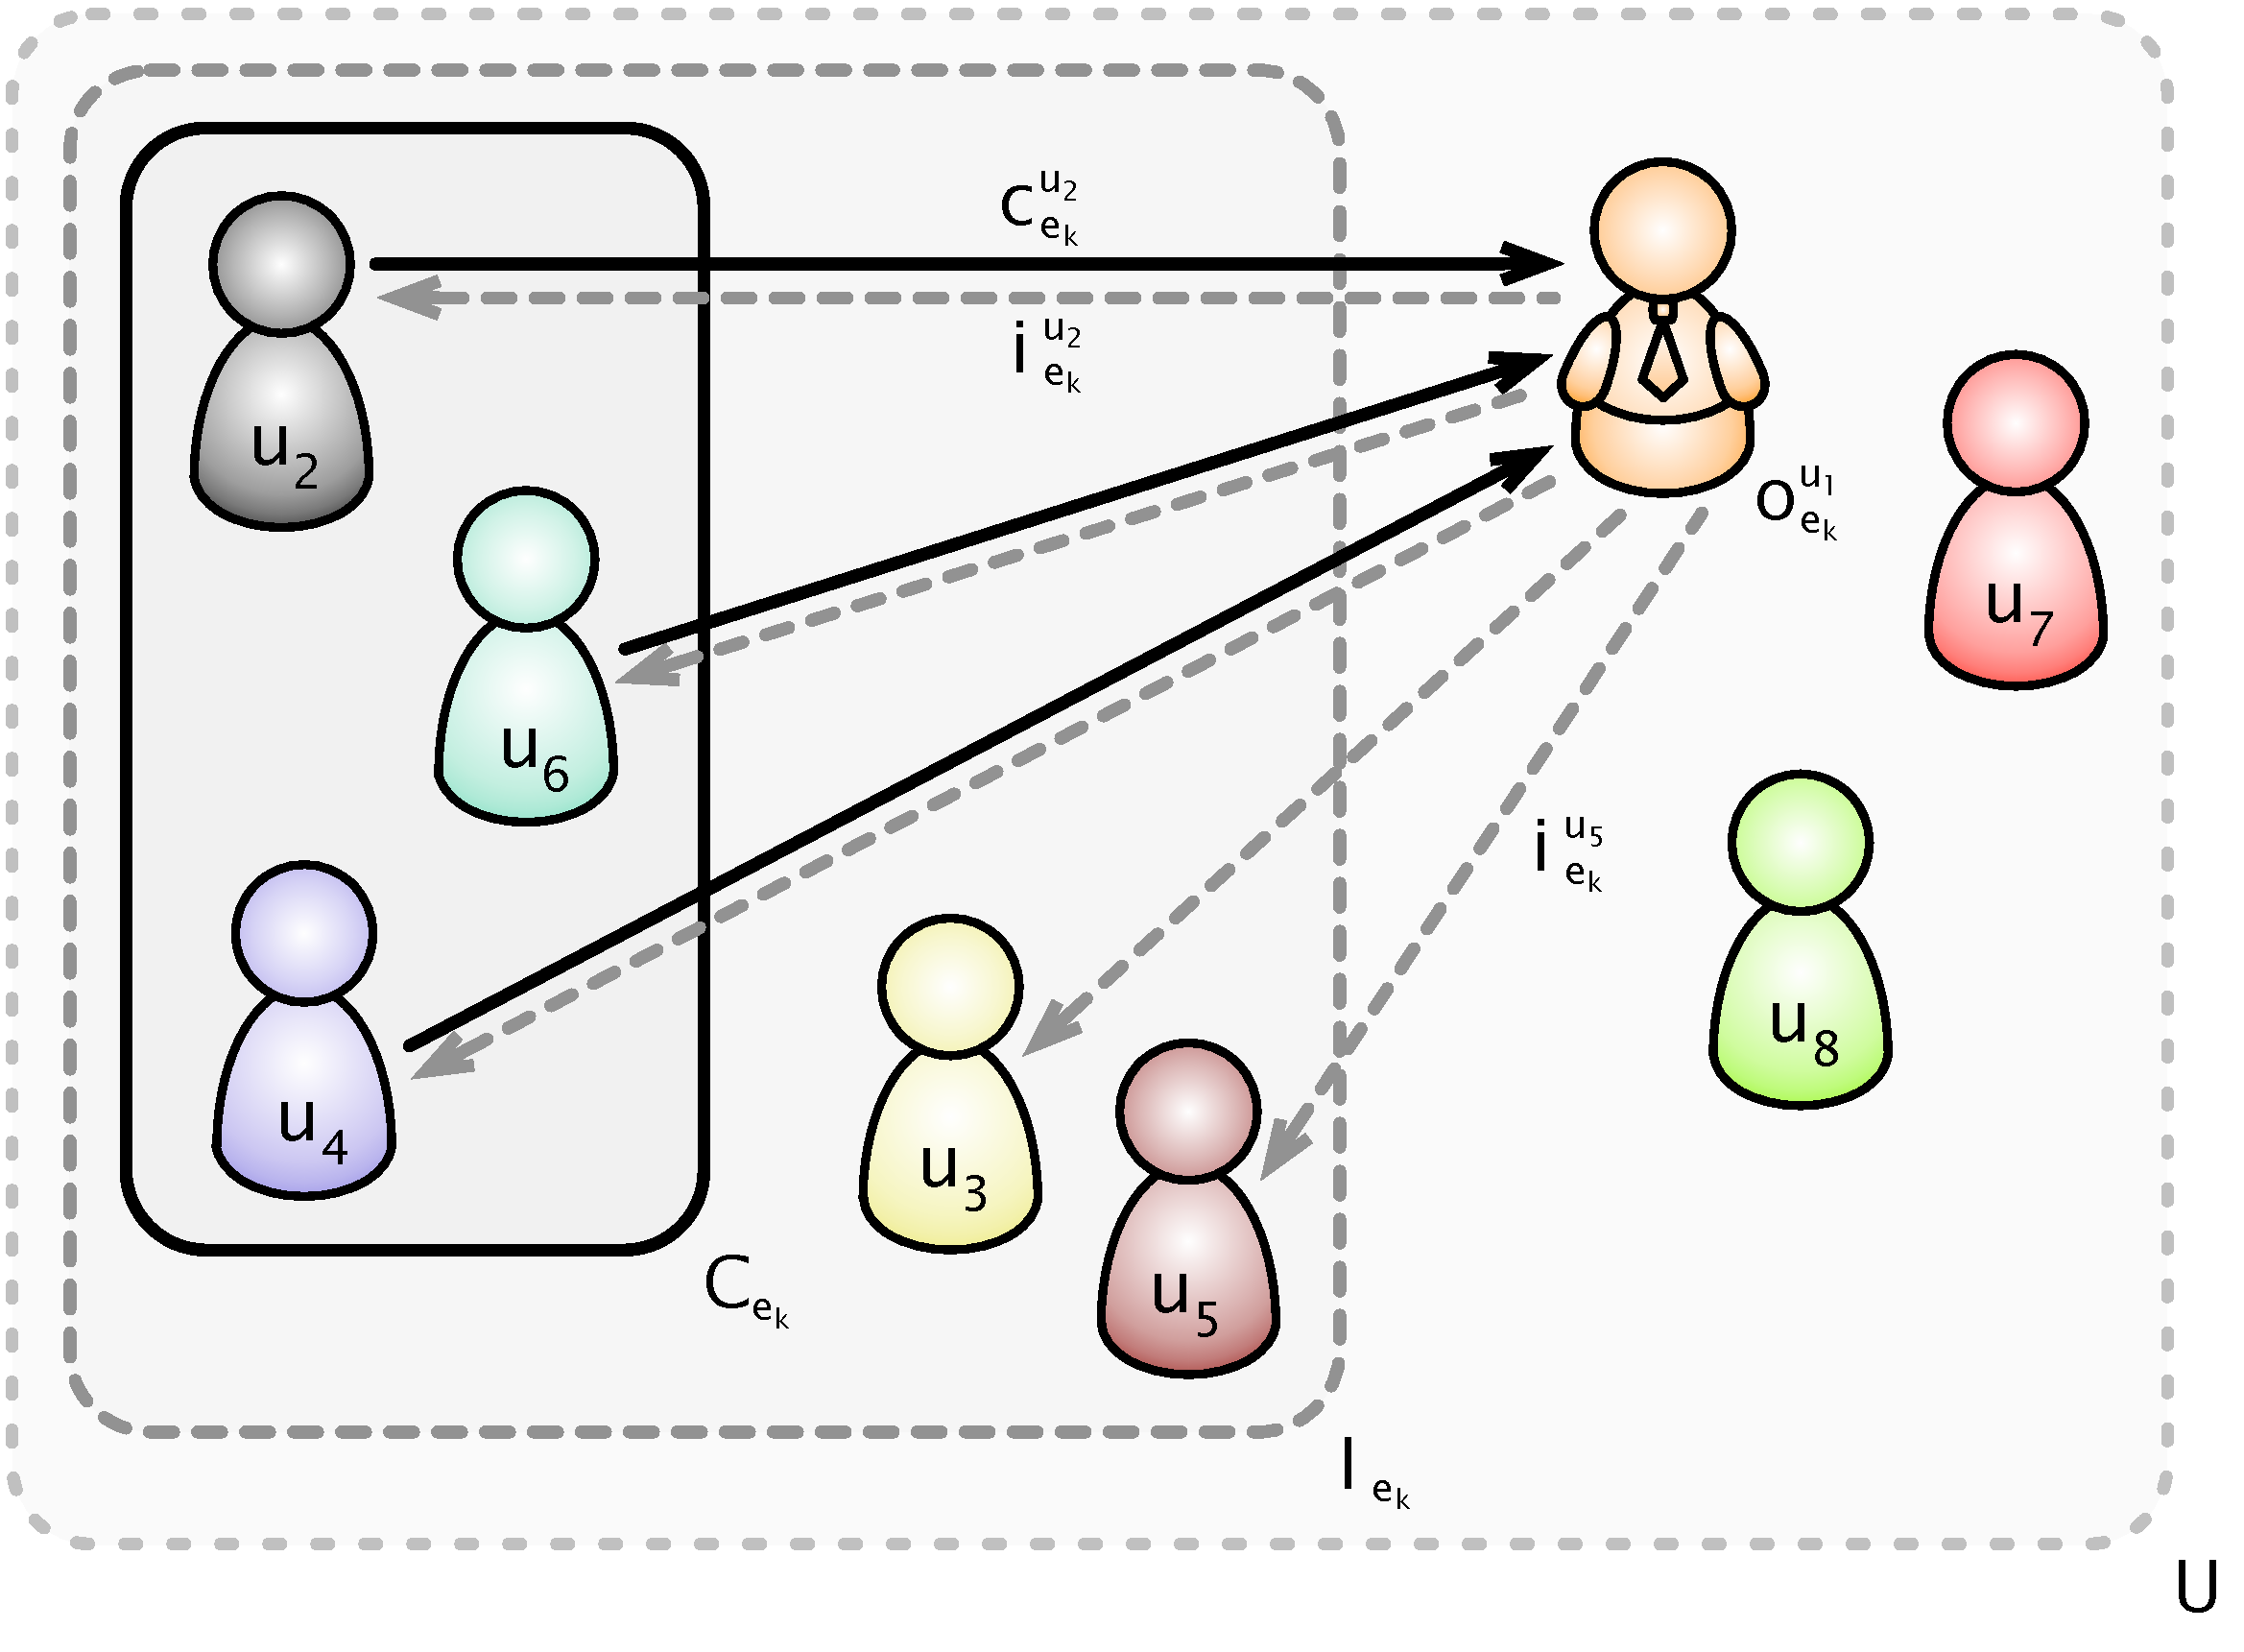
\includegraphics[width=.4\textwidth]{system-overview}
  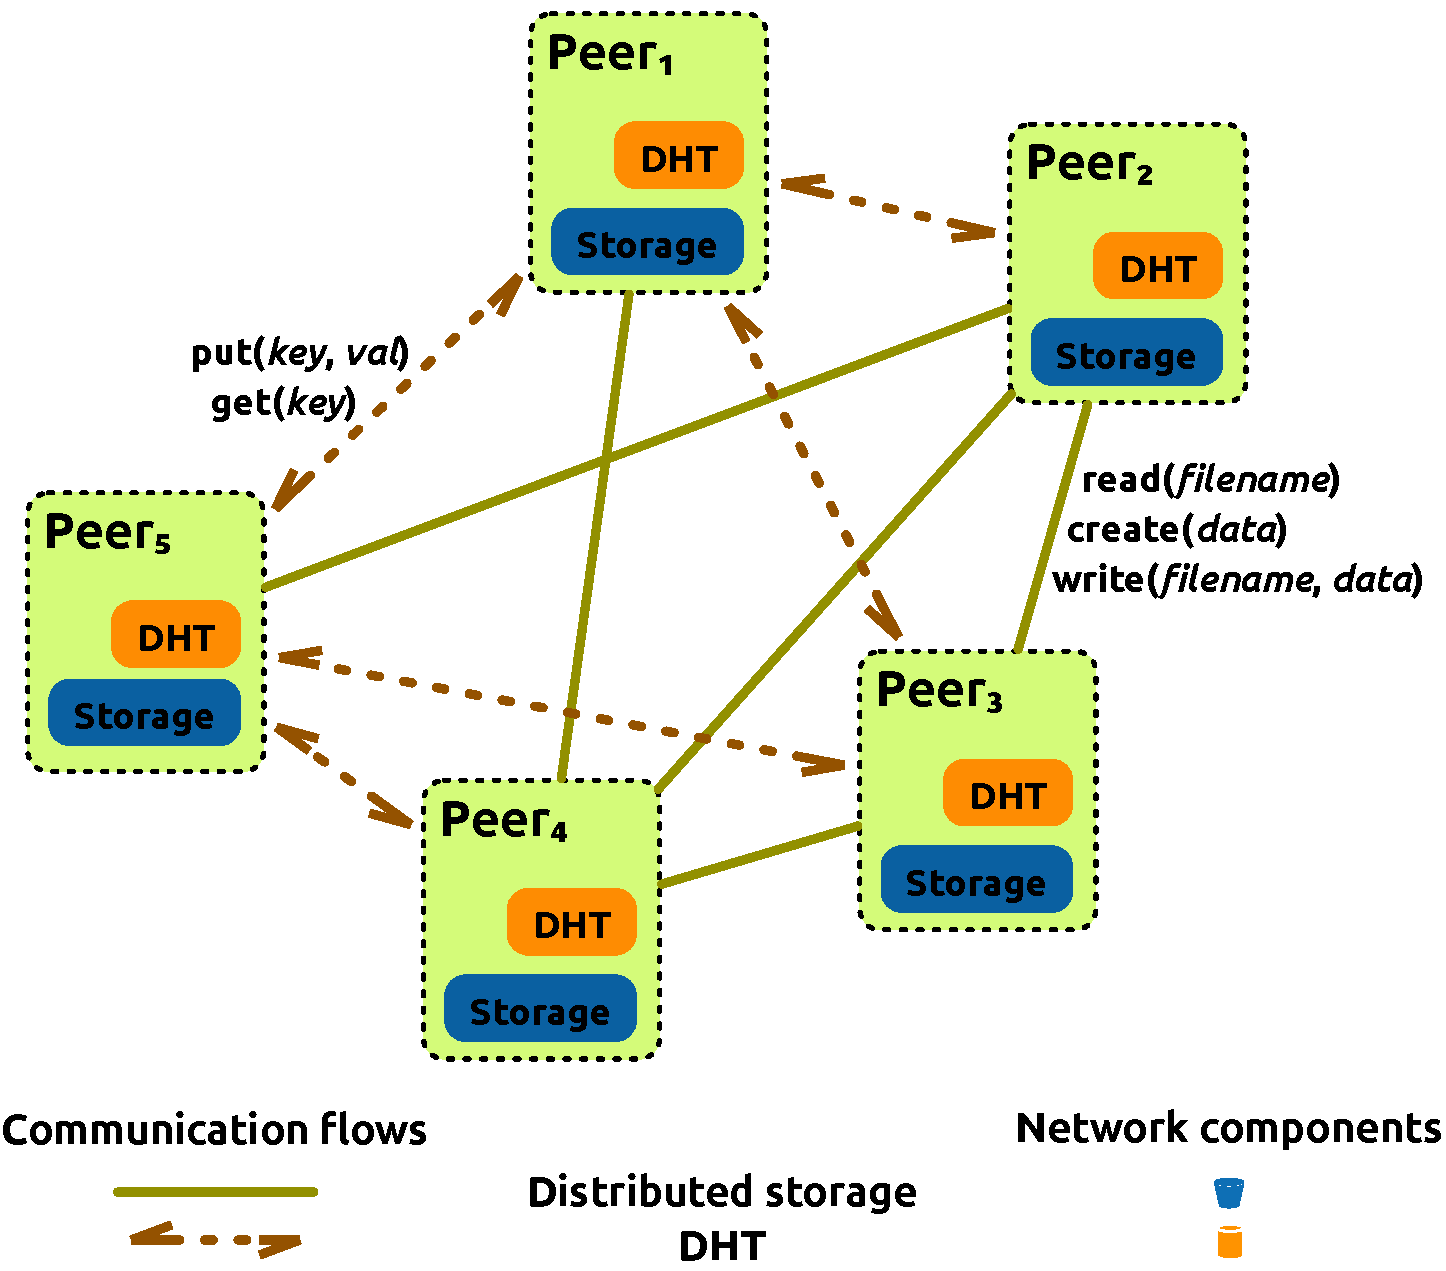
\includegraphics[width=.88\textwidth]{images/passwords-peer-to-peer/system-overview-fully-distributed}
  %\caption{System components. DHT is drawn separately for simplicity, but is
%also run on peers.}
  \caption{Overview of the system.}
  \figlabel{systemoverview}
\end{figure}

% sonja check if needed: that authenticates via cryptographic keys.
To make the system flexible across different implementations, we require as few non-standard features as
possible. The exception to this is the DHT that handles
account registration, mapping each registered username to a reference
in the storage.  For resilience against account hijacking,
we propose modifying the DHT to be write-once on keys:
once an account has been registered, nobody else can register that
username.

From the DHT we require two operations, \texttt{put}($key$, $value$), and
\texttt{get}($key$). The put operation associates the $value$ with the
$key$, and subsequent get operations on that $key$ will return the $value$.
As the DHT is write-once, a second put operation with the same $key$ will not
affect the system state.

The distributed storage functions for data
manipulation are similar to the DHT, with three
differences: we allow the distributed storage to select the ``filename'' for
us; we require that data can be updated; and we assume (minimalistic) access
control when writing. We refer to what is stored in the distributed storage as
files, to simplify our description. While the storage component
can be implemented as a distributed file system, we emphasize that our
requirements are significantly weaker than full file system semantics.

We formalize the API to the storage as having three
operations. First, \texttt{create}($data$) which generates a new file and
returns a filename. Second, \texttt{write}($filename$, $data$) that
overwrites the file $filename$ with content $data$. Third,
\texttt{read}($filename$) which reads the content from a file. Our security
does not require overwritten data to be inaccessible, so a solution
similar to GNUnet~\cite{Bennett03} or
Freenet~\cite{Clarke10} where a new version is stored and
pointed to suffice in our protocols.

We require the storage system to support some minimalistic access control.
Each stored file has an owner, which is the user who created the file.  Only
the owner can perform the \texttt{write} operation. To authenticate ownership
of files, we assume that a public-key cryptographic system is used.

Finally, for the peer sampling component, we require a \texttt{getPeer}() method,
returning a randomly selected peer, with a distribution close to uniform.

\section{Password-based P2P Login} \seclabel{passwordlogin}
For password-based authentication
in P2P systems, the basic functionality involved is registering an account,
and logging in. We also consider password change and remembered logins,
allowing a device to store sufficient information to log in %as a core component 
later without asking for credentials
anew. Following recommendations from the ISO 27002 standard~\cite{iso27002}, we define the
following requirements for our login procedure and add our
own (preceded by a star) to account for several devices.
\begin{itemize}
\item passwords should neither be stored nor transmitted in clear text
\item a user should be able to choose her own passwords and change them
\item files with passwords should be stored separately from application data 
\item[$\star$] a user should use the same password to log in from any device
\item[$\star$] it should not be possible to recover a password by stealing a
device with remembered credentials
\item[$\star$] it should be possible to block access to the account from a
stolen device
\end{itemize}
The standard also defines limitations for password login procedures
that our system cannot provide fully due to the lack of rate-limiting
possibilities in P2P networks: to limit the number of unsuccessful
login attempts and the maximum and minimum time allowed for the
login procedure.  Adapting a multi-party password hardening scheme
\cite{FordK00} could, in future work, be a way to achieve similar
properties in a P2P network. Besides this limitation, our protocols
fulfill the requirements as outlined in the standard, and our
own added requirements.
% According
%to the standard, \emph{the strength of user identification and authentication should be suitable to the sensitivity of the information to be accessed}.


% \textit{\textbf{ISO/IEC 27002:2005}} \\
% \textit{
% 11.5.1 Secure log-on procedures \\
% Access to operating system should be controlled by secure log-on procedure. ... A good log-on procedure should:
% }
% \textit{
% \begin{enumerate}
% \item not display system or application identifiers until the log-on procedure has been successfully completed;
% \item display a general notice warning that the computer should only be accessed by authorized users;
% \item not provide help messages during the log-on procedure that would aid an authorized user;
% \item validate the log-on information only on completion of all input data.If an error condition arises, the system should not indicate which part of the data is correct or incorrect;
% \item limit the number of unsuccessful log-on attempts allowed, e.g. to three attempts, and consider:
% \begin{enumerate}
% \item recording unsuccessful and successful attempts
% \item forcing a time delay before further log-on attempts are allowed or rejecting any further attempts without specific authorization
% \item disconnect data link connection
% \item sending an alarm message to the system console if the maximum number of log-on attempt is reached
% \end{enumerate}
% \item limit the maximum and minimum time allowed for the log-on procedure. If exceeded, the system should terminate the log-on;
% \item display the following information on completion of a successful log-on:
%  \begin{enumerate}
%  \item date and time of the previous successful log-on
%  \item details of any unsuccessful log-on attempts since the last successful log-on
% \end{enumerate}
% \item not display the password being entered or consider hiding the password characters by symbols;
% \item not transmit passwords in clear text over a network;
% \end{enumerate}
% }
% \textit{
% 11.5.2 User identification and authentication \\
% Other information}
% \textit{
% Passwords are a very common way to provide identification and authentication based on a secret that only the user knows. ... The strength of user identification and authentication should be suitable to the sensitivity of the information to be accessed.
% }

\begin{table}[htb]
\centering
\caption{Protocol Terminology}
\tablabel{terminology}
    \begin{tabular}{lp{5.92cm}}
 		\toprule
%		Designator & Description\\
%		\midrule
		$uname$ & Username\\
		$passwd$ & Password\\
		$salt$ & Random byte string\\
		$K_W$ & Cryptographic key for write authentication \\
		$F_{KS}$ & Key store file\\
		$f_{KS}$ & File name of $F_{KS}$\\
		$K_{KS}$ & Cryptographic key (used to encrypt $F_{KS}$)\\
		$F_{LI}, f_{LI}, K_{LI}$ & Login information file, its file name and key\\
		$F_{DL}, f_{DL}, K_{DL}$ & Device login information file, its file name and key\\
		$D, D_{ID}$ & User device and the identifier of $D$\\
		$K_{x1}, K_{x2}, \dots$ & Cryptographic keys for usage after logging in\\
		$devmap$ & Mapping from device identifiers to device login information files and corresponding keys\\
		\bottomrule
    \end{tabular}
\end{table}

We now describe our protocols based on the system model from
\secref{systemsoverview}.  \figref{loginProcedure} shows the
information objects and their storage locations, with arrows for the
abstract flow of the login procedure, \tabref{terminology} lists the terms
used in the algorithms.

\begin{figure}
  \centering
	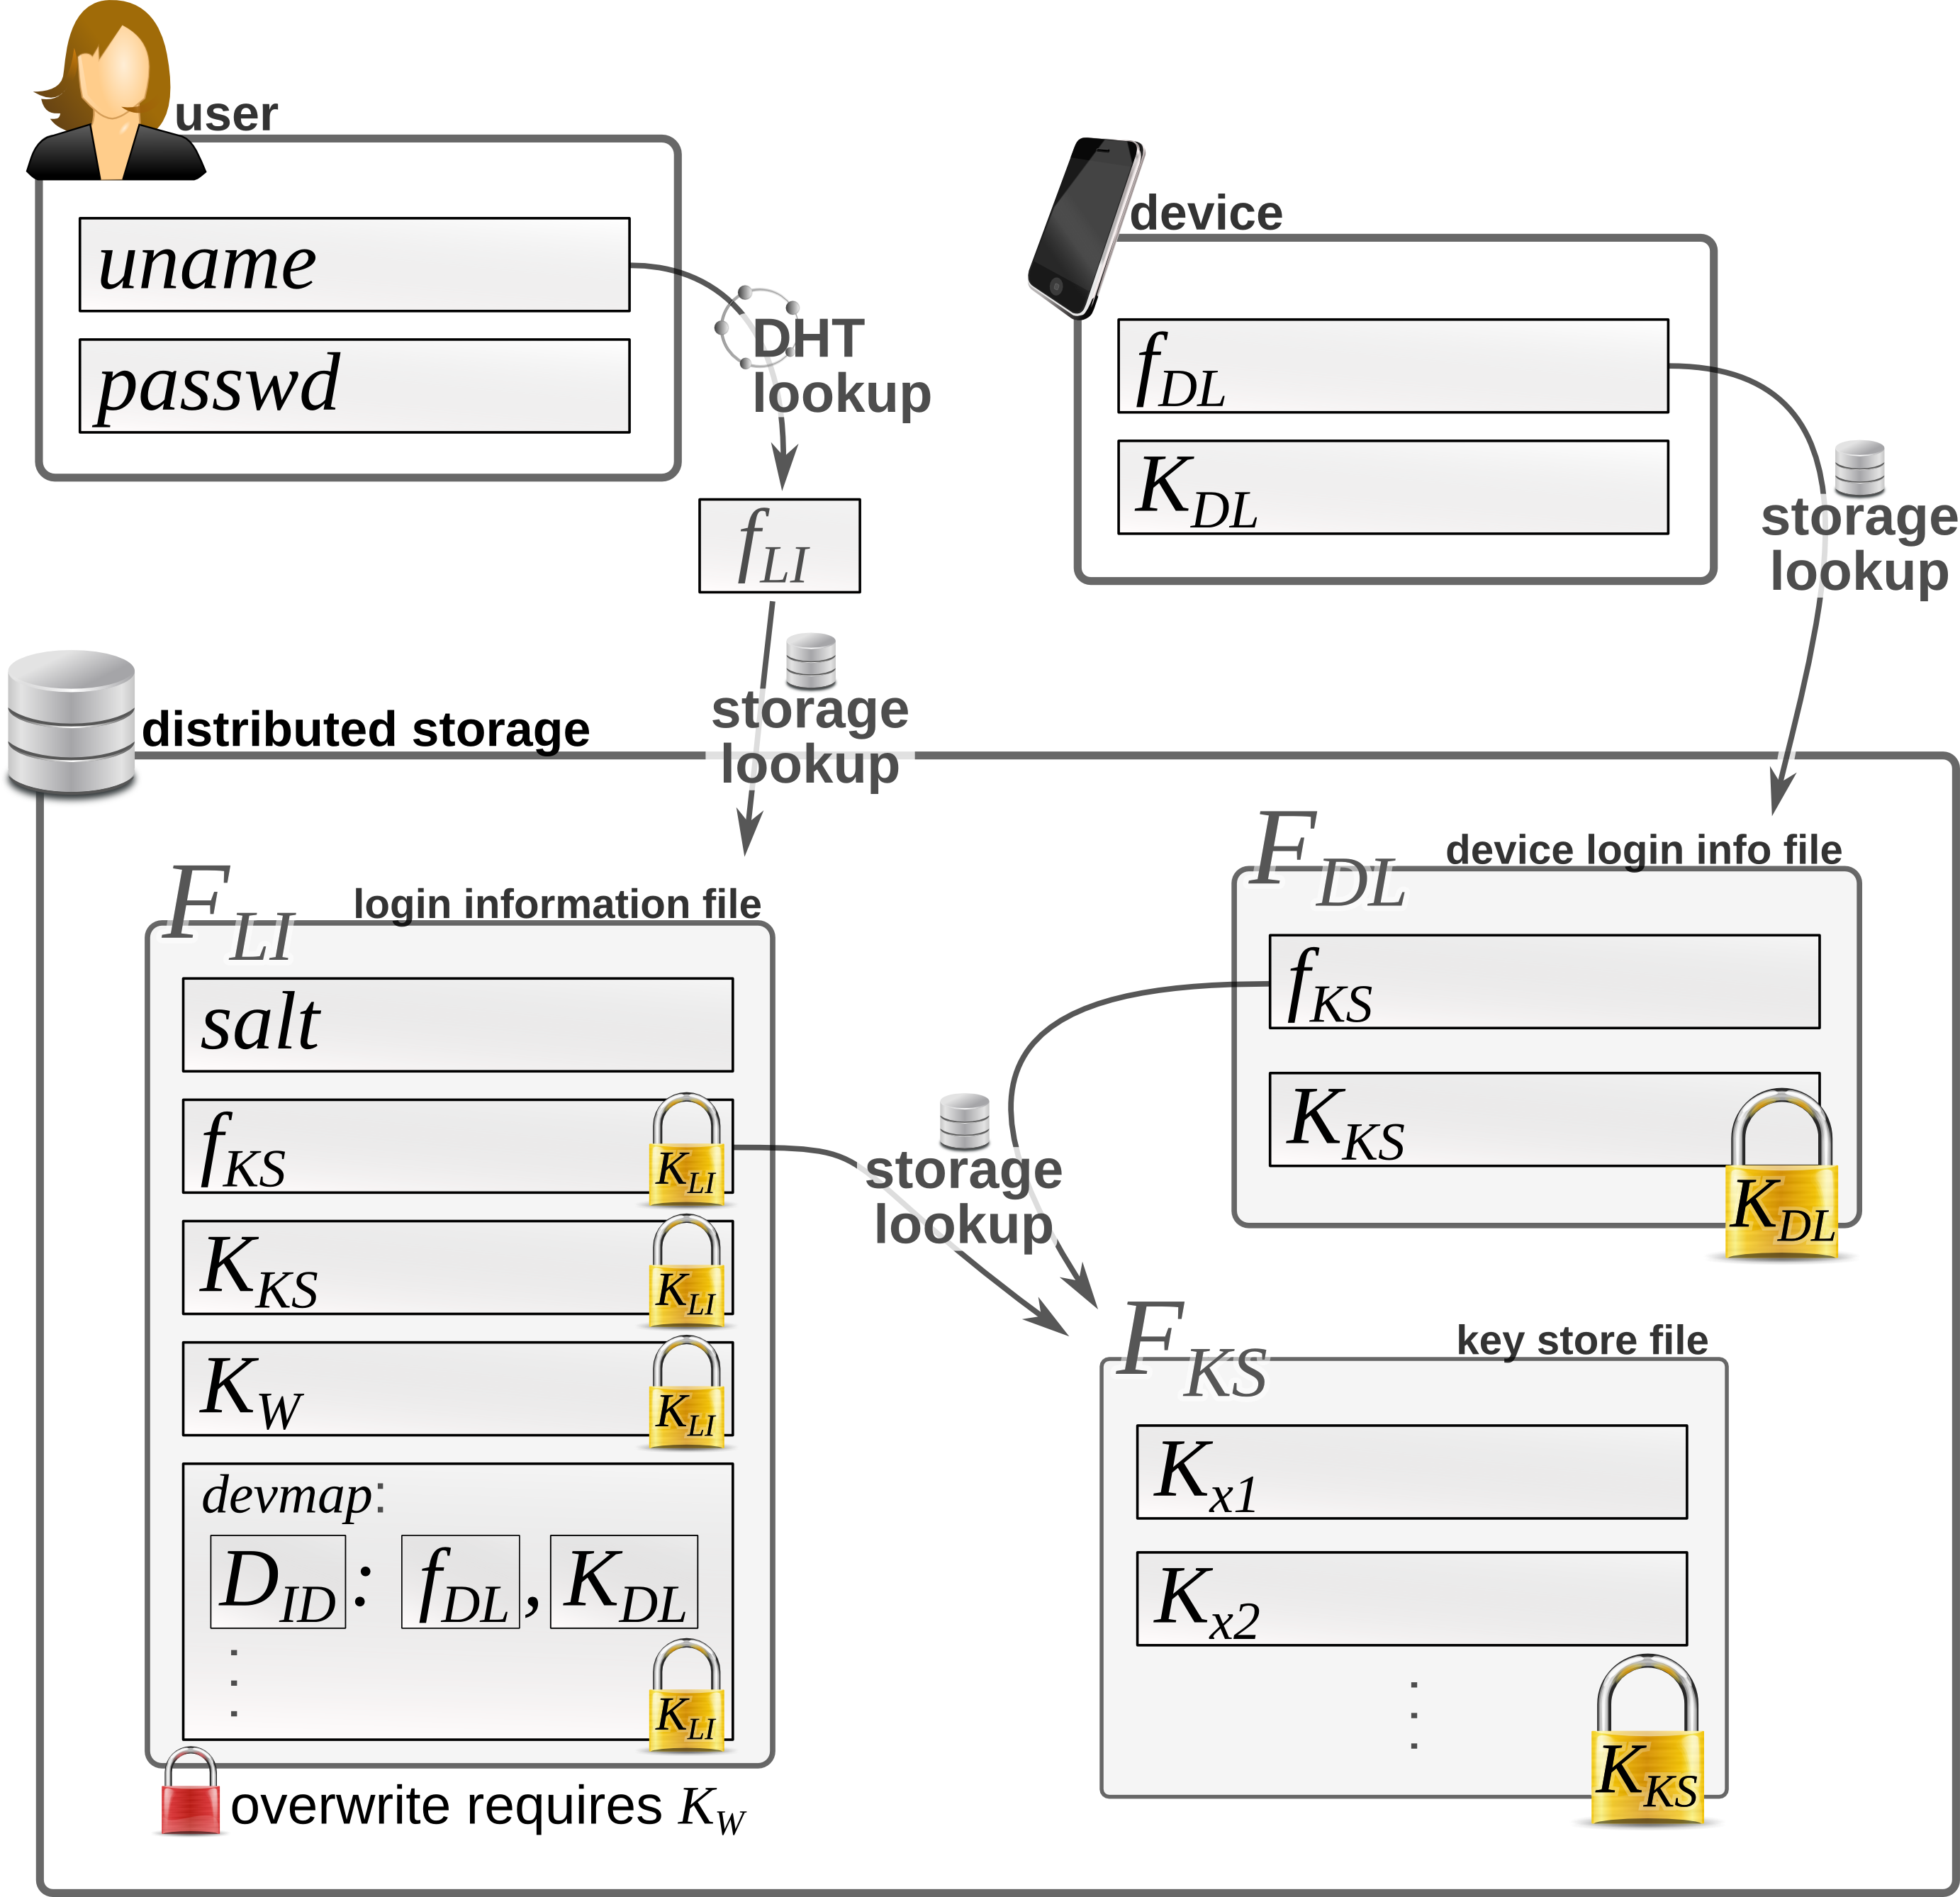
\includegraphics[width=.88\textwidth]{images/passwords-peer-to-peer/user-files-devices}
  \caption{Storage Locations (boxes) and Login Procedure (arrows)}
  \figlabel{loginProcedure}
\end{figure}

%% Pseudocode Definitions
% layout
\newcommand{\LineNumFrequency}{1} % 0 for no line numbers
\algrenewcommand{\algorithmiccomment}[1]{\hfill\textcolor{gray}{// #1}} % comment style
\algnewcommand\Input{\item[\textbf{Input:}]} % define \Input
\algnewcommand\Stored{\item[\textbf{Stored:}]} % define \Stored
% functions
\newcommand{\UserInput}[1]{User.input(``#1'')} % text
\newcommand{\DHTRead}[1]{DHT.get(#1)} % key
\newcommand{\DHTWrite}[2]{DHT.put(#1,#2)} % key, value
\newcommand{\StorageRead}[1]{Storage.read(#1)} % name
\newcommand{\StorageCreate}[1]{Storage.create(#1)} % value
\newcommand{\StorageWrite}[2]{Storage.write(#1,#2)} % name, value
\newcommand{\DeviceLocalRead}{Device.readLocalStore()}
\newcommand{\DeviceLocalWrite}[1]{Device.writeLocalStore(#1)} % value
\newcommand{\DeviceID}{Device.ID}
\newcommand{\NewKey}{generateKey()}
\newcommand{\NewSalt}{generateSalt()}
\newcommand{\NewMap}{createMap()}
\newcommand{\Encrypt}[2]{encrypt$_{#2}$(#1)} % plaintext, cryptkey (without $$)
\newcommand{\Decrypt}[2]{decrypt$_{#2}$(#1)} % ciphertext, cryptkey (without $$)
\newcommand{\KDF}[2]{KDF(#1,#2)} % salt, password
\newcommand{\NewShares}[3]{createShares(#1,#2,#3)} % n, m, plaintext
\newcommand{\UseShares}[1]{useShares(#1)} % shares
\newcommand{\GetPeer}{getPeer()}
\newcommand{\SendMail}[2]{sendMail(#1,#2)} % recipient, content

\subsection{Account Registration} \seclabel{accountregistration}

To register a new account (see \algoref{register}), the user first has to choose
a username $uname$ 
and a password $passwd$.
Next, the user creates a key store file $F_{KS}$, containing all the keys used 
by the P2P application the user wants to log in to (and an additional storage 
key, authenticating write operations on this file). %bgre: not mentioned in the code (if mentioned, it should also be included in the password change protocol)
The user then creates a symmetric key $K_{KS}$, encrypts the file content with this key and puts the ciphertext into the storage, obtaining a file name $f_{KS}$.
Now, the user creates a login information file $F_{LI}$ by creating a random byte string $salt$, deriving a symmetric key $K_{LI}$ from the password $passwd$ and the $salt$, encrypting $f_{KS}$, $K_{KS}$ and $K_W$ (a generated storage key, required for overwriting $F_{LI}$ later) with $K_{LI}$. The salt and the three encrypted values are put into the storage, obtaining a file name $f_{LI}$.
The salt is stored in plaintext, so that the user later can derive the decryption key $K_{LI}$ by only providing the password.
Finally, the user performs the write-once operation \texttt{put} on the DHT
with $uname$ as key and $f_{LI}$ as value. If the username was taken, the user
is prompted for a new username.
Once all operations have succeeded, the user is registered in the system.

\begin{algorithm}
\caption{Account Registration}
\algolabel{register}
% define Do-While construct
\algblockdefx{Do}{While}%
    {\textbf{do}}%
    [1]{\textbf{while} #1}
\begin{algorithmic}[\LineNumFrequency]
 \State $uname \gets$ \UserInput{Choose username:}
\State $passwd \gets$ \UserInput{Choose strong password:}
\State $K_{KS} \gets$ \NewKey % generate keystore key
\State $F_{KS} \gets$ \Encrypt{$K_{x1}||K_{x2}||\dots$}{K_{KS}} % encrypt key material to be stored in key store
\State $f_{KS} \gets$ \StorageCreate{$F_{KS}$} % no need for a storage authenticating key here, because we never need to overwrite this file again (we create new ones instead)
\State $salt \gets$ \NewSalt
\State $devmap \gets$ \NewMap %bgre: for metadata-privacy reasons a new ``empty'' map should consist of a couple of dummy entries
\State $K_{LI} \gets$ \KDF{$salt$}{$passwd$}
\State $K_W \gets$ \NewKey \Comment{suitable for the storage system} % or even provided by the storage system component
\State $F_{LI} \gets salt || $\Encrypt{$f_{KS}||K_{KS}||K_W||devmap$}{K_{LI}}
\State $f_{LI} \gets$ \StorageCreate{$F_{LI}$}\Comment{using $K_W$} %setting ownership using $K_W$
\While{\DHTWrite{$uname$}{$f_{LI}$} fails}
    \State $uname \gets$ \UserInput{Choose new username:}
\EndWhile
\end{algorithmic}
\end{algorithm}


\subsection{Login} \seclabel{loginprotocol}

Once registered, a user is able to log in -- that is, to retrieve the
cryptographic keys stored in the key store file $F_{KS}$ -- 
from any device by only entering her username and password (see \algoref{login}).
%
A \texttt{get} request with the parameter $uname$ to the DHT results in the 
filename $f_{LI}$ for the login information file $F_{LI}$. 
This file is retrieved from the distributed storage and contains the $salt$ in plaintext.
The latter is fed into a key-derivation function together with the user password to derive the key $K_{LI}$.
This key allows the user to decrypt all other content of the login information file,
including the filename $f_{KS}$ of the key store file and the corresponding key $K_{KS}$.
Finally, the user fetches the key store file $F_{KS}$ from the storage system 
and decrypts it, using $K_{KS}$. 
This concludes the login procedure as the user is now in possession
of the keys $K_{x1}, K_{x2}, \dots$, required by the P2P application.

If the user chose to remember the login information on the local device,
a new device login information file $F_{DL}$ is created and saved to the storage system
(which returns a filename $f_{DL}$). This file contains the filename
$f_{KS}$ of the key store file as well as the according key $K_{KS}$ and is encrypted
with a new key $K_{DL}$. On the device, only the filename $f_{DL}$ and the key $K_{DL}$
are stored locally.
Additionally, a reference to the device login information file is stored in the $devmap$ value
of the login information file $F_{LI}$. It contains a mapping from a device identifier to the filename
and key of the device login information file, allowing password changes and device revocation 
as described later.

When the user wants to log in from the same device again, the
locally stored values ($f_{DL}, K_{DL}$) are used to retrieve the device login
information file, decrypt it, and thereby gain access to the key store
file. Thus, the remembered login feature allows the user to log in
without entering the password, while nothing password-related is
stored on the device. Furthermore, remembered logins remain valid
even if the P2P application changes keys in the key store file.

\begin{algorithm}
\caption{Login}
\algolabel{login}
\begin{algorithmic}[\LineNumFrequency]
\State $f_{DL},K_{DL} \gets$ \DeviceLocalRead
\If {$f_{DL} \neq$ \texttt{NULL}} \Comment{non-interactive login}
   \State $F_{DL} \gets$ \StorageRead{$f_{DL}$}
   \State $f_{KS},K_{KS} \gets$ \Decrypt{$F_{DL}$}{K_{DL}}
   \State $saveLoginLocally \gets$ \texttt{False}
\Else \Comment{interactive login}
   \State $uname \gets$ \UserInput{Enter username:}
   \State $passwd \gets$ \UserInput{Enter password:}
   \State $saveLoginLocally \gets$ \UserInput{Remember?}
   \State $f_{LI} \gets$ \DHTRead{$uname$}
   \State $F_{LI} \gets$ \StorageRead{$f_{LI}$}
   \State $salt \gets F_{LI}.salt$ \Comment{stored in plaintext} 
   \State $K_{LI} \gets$ \KDF{$salt$}{$passwd$}
   \State $f_{KS}, K_{KS}, K_W, devmap \gets$ \Decrypt{$F_{LI}$}{K_{LI}}
\EndIf

\State $F_{KS} \gets$ \StorageRead{$f_{KS}$}
\State $K_{x1},K_{x2},\dots \gets$ \Decrypt{$F_{KS}$}{K_{KS}}

\If {$saveLoginLocally$}
   \State $K_{DL} \gets$ \NewKey
   \State $F_{DL} \gets$ \Encrypt{$f_{KS} || K_{KS}$}{K_{DL}}
   \State $f_{DL} \gets$ \StorageCreate{$F_{DL}$}
   \State \DeviceLocalWrite{$f_{DL} || K_{DL}$}
   \State $devmap$.append(\DeviceID, $f_{DL} || K_{DL}$)
   \State $F_{LI} \gets salt || $\Encrypt{$f_{KS}||K_{KS}||K_W||devmap$}{K_{LI}}
   \State \StorageWrite{$f_{LI}$}{$F_{LI}$} \Comment{using $K_W$}
\EndIf

\end{algorithmic}
\end{algorithm}

\subsection{Password Change} \seclabel{pwchangeprotocol}
Before the user can change the password, she must log in using her password to obtain $K_{LI}$.
With this information, the password change can be accomplished (see
\algoref{passwordChange}): the user is asked for a new password and a new salt is generated. The key-derivation function is used to generate a new key $K_{LI}^{new}$ for the login information file. Then, the content of the key-store file is fetched and decrypted (with the old key). A new key $K_{KS}^{new}$ is generated and used for encrypting the key-store content again before it is saved to the storage system, obtaining a new filename $f_{KS}^{new}$. Finally, the login information file is updated: $f_{KS}^{new}, K_{KS}^{new}$, the write credential $K_W$ as well as a new empty device mapping $devmap^{new}$ are encrypted with the new key $K_{LI}^{new}$. Together with the new salt, this ciphertext is written to the distributed storage, using the reference $f_{LI}$ and the credential $K_W$, to authenticate the \texttt{write} operation.
Lastly, the keys stored in the key store should be updated by the application
using our P2P protocol. See \secref{refreshkeystore} for a discussion. At this
point, old device login information files can also be deleted from the storage to
reclaim space.

\begin{algorithm}
\caption{Password Change}
\algolabel{passwordChange}
\begin{algorithmic}[\LineNumFrequency]
\Input $uname, K_{LI}^{old}$
% \State $uname \gets$ \UserInput{Enter username:}
% \State $K_{LI}^{old} \gets$ recovery($uname$) % the recovery function will ask for more user input (e-mail or security-questions)
\State $f_{LI} \gets$ \DHTRead{$uname$}
\State $F_{LI}^{old} \gets$ \StorageRead{$f_{LI}$}
\State $f_{KS}^{old},K_{KS}^{old},K_W,devmap^{old} \gets$ \Decrypt{$F_{LI}^{old}$}{K_{LI}^{old}} 
\State $passwd^{new} \gets$ \UserInput{Enter new password:}
\State $salt^{new} \gets$ \NewSalt
\State $K_{LI}^{new} \gets$ \KDF{$salt^{new}$}{$passwd^{new}$}
\State $devmap^{new} \gets$ \NewMap

\State $F_{KS}^{enc-old} \gets$ \StorageRead{$f_{KS}^{old}$}
\State $F_{KS} \gets$ \Decrypt{$F_{KS}^{enc-old}$}{K_{KS}^{old}}
\State $K_{KS}^{new} \gets$ \NewKey
\State $F_{KS}^{enc-new} \gets$ \Encrypt{$F_{KS}$}{K_{KS}^{new}}
\State $f_{KS}^{new} \gets$ \StorageCreate{$F_{KS}^{enc-new}$} % overwriting the old file (instead of creating a new one) would break the transactional property of this operation 
\State $F_{LI}^{new} \gets$
\Statex $salt^{new} ||$ \Encrypt{$f_{KS}^{new}||K_{KS}^{new}||K_W||devmap^{new}$}{K_{LI}^{new}}
\State \StorageWrite{$f_{LI}$}{$F_{LI}^{new}$} \Comment{using $K_W$}
\State Refresh keys stored in key store
\State Old device login information files may be deleted
\end{algorithmic}
\end{algorithm}


% \begin{algorithm}
% \caption{Password Change} % implies logging out all remembered devices
% \algolabel{passwordChange}
% \begin{algorithmic}[\LineNumFrequency]
% \State $uname \gets$ \UserInput{Enter username:}
% \State $passwd^{old} \gets$ \UserInput{Enter old password:}
% 
% % LOGIN($uname, passwd^{old}$) >>> $K_W,K_{KS},f_{KS}$ 
% \State $f_{LT} \gets$ \DHTRead{$uname$}
% \State $F_{LI} \gets$ \StorageRead{$f_{LI}$}
% \State $salt \gets F_{LI}.salt$ \Comment{stored in plaintext} 
% \State $K_{LI} \gets$ \KDF{$salt$}{$passwd$}
% \State $f_{KS}^{old}, K_{KS}^{old}, K_W, devmap \gets$ \Decrypt{$F_{LI}$}{K_{LI}}
% 
% % \State $passwd^{new} \gets$ \UserInput{Enter new password:") 
% 
% % RESET-PASSWD($uname, passwd^{new}$)
% \State ...\Comment{continue with ``Password Reset'' protocol in line~3}
% \end{algorithmic}
% \end{algorithm}


\subsection{Logout} \seclabel{logoutprotocol}

To log out from the system, the user does not have to interact with the DHT or
the storage system.  Simply wiping her local cache from application data and
all key material restores the pre-login state.  If the user chose to
remember the login on a device, the corresponding device login information
file $F_{DL}$ can also be deleted from
the storage. % bgre: we need a K_W here for overwriting, how do we get it? Or we create a new credential for each F_DL that we store locally as well (and in the devmap).
%bgre: We can not delete the entry in the devices-mapping in F_LI, because we do not have K_LI to modify this field (asking the user for the password for a simple logout would not be convenient),
% so we leave it in and garbage collect it the next time, when it would be used (a garbage entry is one that can not be decrypted by the K_DL stored in the mapping)

A problem related to logging out is revoking remembered credentials on another
device, \eg a user's stolen phone.
To accomplish this, we first run the password change operation, which 
locks out all devices with remembered logins, because the key store key $K_{KS}$
changed (as well as the filename $f_{KS}$).
Next, we use the device mapping $devmap$ to inform all devices about the
new key (and filename), except the device that is to be revoked. To
inform a device about the change, we update the corresponding values in the device's
login information file $F_{DL}$ which can be accessed from the device by using
the locally stored credentials.

\algoref{logoutOtherDevice} describes this necessary extension.  
After running the password change operation, all devices that should \emph{not} 
be revoked and that have remembered logins (and therefore are 
referenced in the device mapping $devmap$) are processed.
The device login information filename $f_{DL}$ and its key $K_{DL}$ 
are read, and the new key store key $K_{KS}^{new}$ and filename $f_{KS}^{new}$ 
are written to the device login information file $F_{DL}$, encrypted under the 
device key $K_{DL}$. Finally, the modified $devmap$ is saved back to the 
login information file $F_{LI}$.

% We remark that device revocation addresses the problem when a user's device is
% lost. It does not help in case the user has entered her credentials into a
% malicious device, as such a device can store her username and password
% directly.
% \todo{bgre: This paragraph is a bit misleading, because a password change is 
%             part of the logout operation (not necessary but in our protocol),
%             so it is more a race between the malicious device and the user 
%             (who changes password first, wins). So, maybe delete this paragraph 
%             here and say something about the race issue in the security 
%             evaluation instead?}

\begin{algorithm}
\caption{Logout Other Device} % implies changing the password
\algolabel{logoutOtherDevice}
% define For-Each construct
\algblockdefx{Foreach}{Endforeach}%
    [2]{\textbf{foreach} #1 \textbf{in} #2}%
    {\textbf{end}}
\begin{algorithmic}[\LineNumFrequency]
\State ... \Comment{run \algoref{passwordChange} (Password Change)}
\State $deviceToLogout \gets$ \UserInput{Select device:}
\State $devmap.remove(deviceToLogout)$
\Foreach {$D_{ID}$}{$devmap$} \Comment{all devices to keep}
  \State $f_{DL},K_{DL} \gets$ $devmap$.get($D_{ID}$)
  \State $F_{DL} \gets$ \Encrypt{$f_{KS}^{new}||K_{KS}^{new}$}{K_{DL}}
  \State \StorageWrite{$f_{DL}$}{$F_{DL}$}
\Endforeach
\State ... \Comment{save modified $devmap$ back to $F_{LI}$}
\end{algorithmic}
\end{algorithm}

\section{Password Recovery} \seclabel{recovery} An important part of
password-based logins is the possibility for users to recover their
accounts if they forget their passwords. We refer to this as a
\emph{password recovery mechanism}. The goal of a password recovery
mechanism is to provide a secondary way of authenticating the
user. There are a number of password recovery mechanisms used in
practice. In our experience, three of the most common ones are
password hints, security questions, and e-mail based recovery. Other
approaches (beyond the scope of this paper) include vouching for identity by
social contacts~\cite{Brainard06}, or using trusted devices.
% \begin{itemize}
% \item Password hints
% \item Security questions
% \item E-mail based password recovery
% \end{itemize}

Password hints means that the user may enter a hint at the same time as she
sets this password. The hint will be displayed to her if she forgets her
password, and should be selected such that it helps her recall her password,
but does not make it significantly easier for someone else to guess it. The
hint is not truly a secondary authentication mechanism, but rather a means to
recovering the original password-based authentication mechanism. A basic 
version of password hints would be straightforward to implement in our system: 
the hint can be stored in plaintext in the login information file. 
Security questions and e-mail based password recovery are more complex to adapt.
We described their implementation in detail after listing requirements.

As in \secref{passwordlogin} for the login procedure, we  define a set of functional
requirements for password recovery, based on the ISO 27002 standard~\cite{iso27002} as follows. We
also augment the list with requirements of our own (preceded by a star).

\begin{itemize}
	\item establish methods to verify the identity of a user prior to allowing the user to choose a new password
	\item communicate with those affected by or involved with recovery security incidents 
	\item have procedures to allow recovery and restoration of business operations and availability of information in a time-scaled manner 
	\item a legitimate user should be able to recover lost (forgotten) or broken (device's) keys
	\item[$\star$] the recovery procedure should allow a user to set a new password, not reveal the old password
	\item[$\star$] the process of recovery should be easy to use
	\item[$\star$] sensitive information for recovery should be kept secret
\end{itemize}
Our protocols support these requirements. The sole exception is that if a
password is reset via security questions alone, the system would not
``communicate with those affected'' (e.g., send an e-mail notification that
the password had been reset, as is common in centralized services).
We remark that the last item is a stronger property than many
centralized systems provide. In our system, no one learns the
answers to a user's security questions. We consider this to be
important, since many systems use similar security questions.

The operations described in this section imply minor additions to the protocols
of \secref{passwordlogin}, \ie invoking the update procedures after each password change
(to sustain transaction safety, the updates have to be included in the final write operation of
the password change operation).

% \textit{Some properties of interest for password recovery to argue, discuss, include,...:
% \begin{itemize}
% 	\item Entropy
% 	\item Fault-tolerance (what happens with the chosen peers over time... for instance, if they don't ever log in back, we could run into the situation of having less `still-active' peers than the minimum we require to perform the recovery) Check paper: \url{http://dl.acm.org/citation.cfm?id=501985}
% 	\item Minimize delay when recovering (password hint is presumably the fastest one for instance). This is related to evaluation... disaster scenario
% 	\item Collision avoidance. This is related to the distribution of the peers chosen, we now say that it should be almost uniform, but how do we guarantee that? \todo{Look for reference on P2P systems and see how they choose peers to avoid these problems}
% 	\item Usability (minimize complexity for the user, for instance choosing the random peers when using the email recovery could be a hassle...). Unlikely that this one goes in, but found this paper on adaptability of the questions... \url{http://www.comp.lancs.ac.uk/iwssi2007/papers/iwssi2007-04.pdf} \todo{Use this paper also for evaluation, it has details about attacks}
% %Maybe this one too: http://www.sciencedirect.com/science/article/pii/S0167404807001083
% \end{itemize}
% }

\begin{table}[htb]
\centering
\caption{Recovery Protocol Terminology}
\tablabel{recoveryTerminology}
    \begin{tabular}{lp{65mm}}
		\toprule
% 		Designator & Description\\	
% 		\midrule
		\multicolumn{2}{c}{Security Question Recovery}\\
		\midrule
		$qS_i $ & ($n,k$)-secret sharing share of $K_{LI}$\\
		$Q_i $ & Security challenge question\\
		$A_i $ & Answer to question $Q_i$\\
		$qsalt_i $ & Random byte string \\
		$qK_i $ & Key to encrypt the share $qS_i$\\
		\midrule
		\multicolumn{2}{c}{E-mail Based Recovery}\\
		\midrule
		$K_R $ & Long-term recovery key\\
		$eS_i $ & ($n,k$)-secret sharing share of $K_R$\\
		$email $ & Recovery e-mail address of the user\\
		$peer_i $ & Randomly selected peer\\
		$esalt_i $ & Random byte string (to seed the e-mail commitment)\\
		$ksalt_i $ & Random byte string (to seed the key $eK_i$)\\
		$C_i $ & Cryptographic commitment to the e-mail address\\
		$eK_i $ & Key to encrypt the share $eS_i$\\
		\bottomrule
    \end{tabular}
\end{table}

\subsection{Security Questions}

Security questions is a password recovery technique
that relies on answers to questions the user is asked during registration.
The answers should be such that they cannot be easily guessed or researched by an attacker, but
still stable over time, memorable, and definite~\cite{GoodSecurityQuestions}.
Rabkin~\cite{Rabkin08} underlines the importance to choose good questions especially in the era of social networks.
Frykholm and Juels~\cite{FrykholmJ01} discuss a related technique that is similar to 
our adaption of this scheme.  

% One popular technique in centralized systems when a user creates a new account is asking the user with a set of questions such that in the hypothetical case that the user forgets its account password she is still able to regain access to the account by setting up a new password once the answers to those questions asked during registration match to the answers given during registration.

% \textit{This technique, called "Challenge questions" is discussed in the FFIEC supplement to the "Authentication in an Internet Banking Environment" guidance. Ordinary challenge questions are not considered adequate due to the amount of information about people on the Internet, but sophisticated, “out of wallet” questions provide an "effective component of a layered security".}

We assume that the user provides $n$
answers $A_i$ to suitable security questions $Q_i$. In order to recover the password, we 
require the user to answer any $k$ out of these $n$ questions correctly. 
The choice of $k$ constitutes an obvious trade-off between security and usability.
A successful recovery yields the key $K_{LI}$ to the login information file, allowing
the user to change the password, using \algoref{passwordChange}.
Our implementation does not require the user to provide new answers
after a regular password change. Additionally, we avoid storing the plaintext answers to the security questions.

For the setup of the question based recovery mechanism (\algoref{questionSetup}), we first create $n$ 
shares $qS_1, \dots, qS_n$ of the key $K_{LI}$ under an ($n,k$)-secret sharing scheme. For each
of these shares, we create a salt $qsalt_i$, derive a key $qK_i$ from this salt and the
answer $A_i$, and use it to encrypt the share, yielding $qS_i^{enc}$. Furthermore we encrypt the key $qK_i$
with the login information file key $K_{LI}$, for the update procedure described later.
Finally, the login information file is extended with all questions $Q_i$, the salts $qsalt_i$, the encrypted
shares $qS_i^{enc}$ and the encrypted keys $qK_i^{enc}$. When recovering, the
user has to reproduce at least $k$ answers, which together with the stored
salts can be used to derive $k$ keys $qK_i$, which in turn can decrypt $k$
shares $qS_i$.

When $K_{LI}$ changes (\eg due to a regular password change), we update the recovery information
as in \algoref{questionUpdate}: for the new key $K_{LI}^{new}$, a new set of shares is created.
Next, the keys $qK_i$ are decrypted and used to encrypt the new shares. Neither the keys
$qK_i$ nor the salts $salt_i$ change, so the user can still use the same answers for recovery. Finally, the updated
shares (and re-encrypted keys, to allow further updates) are saved back to the login information file.

\begin{algorithm}
\caption{Security Questions Setup}
\algolabel{questionSetup}
\begin{algorithmic}[\LineNumFrequency]
\State $qS_1,\dots,qS_n \gets$ \NewShares{$n$}{$k$}{$K_{LI}$} 
\For{$i \gets 1, n$}
  \State $Q_i \gets$ \UserInput{Enter question $i$:}
  \State $A_i \gets$ \UserInput{Enter answer $i$:}
  \State $qsalt_i \gets$ \NewSalt
  \State $qK_i \gets$ \KDF{$qsalt_i$}{$A_i$}
  \State $qS_i^{enc} \gets$ \Encrypt{$qS_i$}{qK_i}
  \State $qK_i^{enc} \gets$ \Encrypt{$qK_i$}{K_{LI}}
\EndFor
\State add to $F_{LI}$: $qS_i^{enc},qK_i^{enc}$ and the plaintext values of $Q_i,qsalt_i \quad\forall i \in \{1,\dots,n\}$ 
\end{algorithmic}
\end{algorithm}

\begin{algorithm}
\caption{Security Questions Update (on $K_{LI}$ change)}
\algolabel{questionUpdate}
\begin{algorithmic}[\LineNumFrequency]
\State $qS_1^{new},\dots,qS_n^{new} \gets$ \NewShares{$n$}{$k$}{$K_{LI}^{new}$}
\For{$i \gets 1, n$}
  \State $qK_i \gets$ \Decrypt{$qK_i^{enc}$}{K_{LI}}
  \State $qS_i^{new-enc} \gets$ \Encrypt{$qS_i^{new}$}{qK_i}
  \State $qK_i^{new-enc} \gets$ \Encrypt{$qK_i$}{K_{LI}^{new}}
\EndFor
\State update in $F_{LI}$: $qS_i^{new-enc},qK_i^{new-enc} \quad\forall i \in \{1,\dots,n\}$ 
\end{algorithmic}
\end{algorithm}

\subsection{E-mail Based}

In e-mail based password recovery, the user is sent an e-mail
containing some information, typically a link with a token, by which she can
reset her password. This link is sent to an e-mail address she has registered
with her account.

We adapt this scheme by randomly choosing a number of peers, that collaboratively provide this
functionality to the user. We use ($n,k$)-secret sharing 
to enable password recovery even if not all of the involved peers are online
when the user wants to recover the password. We discuss parameter choices of $k$ and $n$
in \secref{evalemail}.

To provide persistence of the recovery mechanism independent of a changing key $K_{LI}$ 
(\eg due to a password change), the result of the recovery process is a 
recovery key $K_R$, that always encrypts the current version of $K_{LI}$. 
\algoref{emailSetup} describes the setup procedure: 
From the recovery key $K_R$, $n$ shares $eS_1,\dots,eS_n$ are generated using ($n,k$)-secret
sharing. For each share, a random peer $peer_i$ is picked, two salts $esalt_i$ and $ksalt_i$ are created and a cryptographic commitment $C_i$
is derived from the salt $esalt_i$ together with the $email$. This commitment will be used to authorize the
user to the peer, and bind it to this specific e-mail address. 
Next, a key $eK_i$, to encrypt the share $eS_i$, is derived in the same way as the commitment, 
but with salt $ksalt_i$. 
A different salt is needed so that the peer cannot decrypt the share (before learning the address).
The commitment and the encrypted share are stored at the peer. The login information $F_{LI}$ file is extended
with a list of the chosen peers $peer_i$ and the according salts $esalt_i$, $ksalt_i$, as well as $K_{LI}^{enc}$,
encrypted with the recovery key, and the recovery key, encrypted with $K_{LI}$ (to allow for password changes).


\begin{algorithm}
\caption{E-mail Recovery Setup}
\algolabel{emailSetup}
\begin{algorithmic}[\LineNumFrequency]
\State $K_R \gets$ \NewKey \Comment{long-term recovery key}
\State $K_{LI}^{enc} \gets$ \Encrypt{$K_{LI}$}{K_R}
\State $eS_1,\dots,eS_n \gets$ \NewShares{$n$}{$k$}{$K_R$} 
\State $email \gets$ \UserInput{Enter recovery e-mail address:}
\For{$i \gets 1, n$}
  \State $peer_i \gets$ \GetPeer
  \State $esalt_i \gets$ \NewSalt
  \State $ksalt_i \gets$ \NewSalt
  \State $C_i \gets$ \KDF{$esalt_i$}{$email$} \Comment{commitment}
  \State $eK_i \gets$ \KDF{$ksalt_i$}{$email$}
  \State $eS_i^{enc} \gets$ \Encrypt{$eS_i$}{eK_i} % share-holders can only collude after the user revealed its email address
  \State store at $peer_i$: $C_i, eS_i^{enc}$  
\EndFor
\State $K_R^{enc} \gets$ \Encrypt{$K_R$}{K_{LI}}
\State add to $F_{LI}$: $K_{LI}^{enc}, K_R^{enc}$ and the plaintext values of $peer_i, esalt_i, ksalt_i \quad\forall i \in \{1,\dots,n\}$ 
\end{algorithmic}
\end{algorithm}


To recover the password (\algoref{emailUser}), the user looks up the available
information in the login information file, including the list of peers 
to be requested for assistance.
Each request is authorized by the commitment $C_i$, that the peer can derive
from the salt $esalt_i$ and the e-mail address, that the user provided (\algoref{emailPeer}).
If the request was legitimate, the peer sends the encrypted share to the e-mail address.
As soon as the user collected $k$ answers, she can recover $K_{LI}$.

\begin{algorithm}
\caption{E-mail Recovery: User}
\algolabel{emailUser}
\begin{algorithmic}[\LineNumFrequency]
\State $uname \gets$ \UserInput{Enter username:}
\State $email \gets$ \UserInput{Enter e-mail:}
\State $f_{LI} \gets$ \DHTRead{$uname$}
\State $F_{LI} \gets$ \StorageRead{$f_{LI}$}
\State $K_{LI}^{enc}; \forall i: peer_i, esalt_i, ksalt_i \gets F_{LI}$ \Comment{plaintext part}
% \State $K_{LI}^{enc}, peer_{1,\dots,n}, esalt_{1,\dots,n}, ksalt_{1,\dots,n} \gets F_{LI}$ \Comment{plaintext part}
\State $\forall i:$ send $(email, esalt_i)$ to $peer_i$ \Comment{send $n$ requests}
\State $eS_1^{enc},\dots,eS_k^{enc} \gets$ read e-mail \Comment{wait for $k$ e-mails}
\For{$i \gets 1, k$}
  \State $eK_i \gets$ \KDF{$ksalt_i$}{$email$}
  \State $eS_i \gets$ \Decrypt{$eS_i^{enc}$}{eK_i}
\EndFor
\State $K_R \gets$ \UseShares{$eS_1,\dots,eS_k$}
\State $K_{LI} \gets$ \Decrypt{$K_{LI}^{enc}$}{K_R}
\State ...\Comment{run \algoref{passwordChange} (Password Change)}
\end{algorithmic}
\end{algorithm}

\begin{algorithm}
\caption{E-mail Recovery: Peer}
\algolabel{emailPeer}
\begin{algorithmic}[\LineNumFrequency]
\Stored $C_i, eS_i^{enc}$ \Comment{stored at peer}
\Input $email, esalt_i$ \Comment{provided by the user request} % note that still the peer cannot decrypt the share, because it does not have ksalt_i to derive eK_i
\If {$C_i =$ \KDF{$esalt_i$}{$email$}} \Comment{legitimate request}
  \State \SendMail{$email$}{$eS_i^{enc}$}
\EndIf
\end{algorithmic}
\end{algorithm}

To provide long-term persistence of this recovery mechanism,
$K_{LI}^{enc}$ has to be updated whenever $K_{LI}$ changes. 
\algoref{emailUpdate}
describes the necessary steps, including updating
$K_R^{enc}$ to allow subsequent updates.

\begin{algorithm}
\caption{E-mail Recovery Update (on $K_{LI}$ change)}
\algolabel{emailUpdate}
\begin{algorithmic}[\LineNumFrequency]
\State $K_R \gets$ \Decrypt{$K_R^{enc}$}{K_{LI}^{old}} 
\State $K_{LI}^{enc-new} \gets$ \Encrypt{$K_{LI}^{new}$}{K_R}
\State $K_R^{enc-new} \gets$ \Encrypt{$K_R$}{K_{LI}^{new}}
\State update in $F_{LI}$: $K_{LI}^{enc-new}, K_R^{enc-new}$ 
\end{algorithmic}
\end{algorithm}




%\subsection{Alternatives Password Recovery Mechanisms}
%\todo{bgre: merge this (1-sentence-)subsection with next one? Or move it to intro of this section?}

\subsection{Combining Approaches}

The approaches presented above can be composed, either sequentially or in
parallel. By sequential composition, we mean that the user must \emph{both}
correctly answer security questions and receive e-mail. By parallel
composition, we mean that either mechanism can be used alone to recover the
password. The latter is achieved by using both systems in parallel.

For sequential composition, the user picks a uniformly random string
$r$ of the same length as $K_{LI}$. The user stores $r$ in one of the
mechanisms, and $K_{LI} \oplus r$ in the second mechanism, where $\oplus$
denotes the exclusive-OR operation. If one recovers both of these,
$K_{LI}$ can be computed. If one learns only one of the pieces, nothing
is gained, as both $r$ and $K_{LI} \oplus r$ are uniformly random.
More generally, to combine $n$ mechanisms in arbitrary ways, ($n,k$)-secret
sharing can be used. What we describe here are two trivial such schemes for $n
= 2$.

\section{Security} \seclabel{security}

%We now turn to the security properties of our proposed protocols. 
The goal we set is to emulate the security provided by a centralized solution. Some security risks are inherent to the password functionality, and
apply regardless of implementation technique. For instance, in e-mail based
recovery, an attacker compromising the victim's e-mail account can reset her
password.

In this section, we elaborate on security concerns of our protocols. We do not
have full cryptographic security proofs of our protocols, something which is
important future work.

Concerning safety, we have designed our protocols such that
persistently stored data remains in a consistent state if the
protocol is aborted at any point. Some protocols may, if an operation
fails, leave orphan files in the storage. If our protocol for revoking
remembered credentials is interrupted, it may revoke more devices than
intended. Apart from this, our operations have transactional semantics,
assuming small writes (both creation, and updates) to the storage are atomic operations and that
operations block until successful.


\subsection{Adversary Model}

To capture the concept of collusions, we consider an adversary 
that corrupts a number of nodes. %We categorize the attacker as either
                                %passive or active. 
Upon corruption, the adversary gains all information known to that
node, and in the case of an active adversary, can also control its future
actions. The adversary can also make requests to the underlying
system, \eg read files from the distributed storage. As almost all our
protocols mainly operate on publicly readable (encrypted) data, this
ability is important. The only computation made by nodes different from the
one logging in are in verifying write operations, and in e-mail based password
recovery.

\subsection{Risks in Used Components}

As our protocols make use of several standard components, vulnerabilities in those 
components can also affect our system. For instance, an adversary may prevent 
a user from logging in by attacking the victim's ability to read her login 
information file from the distributed storage.
We note that there are many security 
techniques in DHTs that can mitigate such threats, and refer 
to Urdaneta\etal~\cite{UrdanetaPS11} for a recent survey.

\subsection{Offline Guessing}

An issue in password authentication based on a (distributed) file system is
that the information required to verify a password attempt is inherently
exposed. This means that in our scheme, we cannot prevent an attacker from
mounting an offline attack against our encrypted passwords. This is a
considerable drawback from centralized schemes, where the encrypted password
database is kept protected.

As a partial mitigation, we utilize a KDF with a per-user salt. This forces an
attacker to evaluate the KDF individually for each user on a password guess,
defeating parallel attacks against multiple users. We recommend the system be
instantiated with a slow KDF, such as bcrypt~\cite{DBLP:conf/usenix/ProvosM99}
to throttle offline guessing. The protocol could be modified to reduce storage
by using the username as a salt, but we recommend against that as it would be
vulnerable to pre-computation (before the system is started, or between
instances using the same KDF) attacks against common username-password pairs.

The problem of a server performing offline attacks against its password
database was treated by Ford and Kaliski~\cite{FordK00}. Their techniques are
client-server based, and require all servers to be online for a login. We
leave it as future work to investigate modifying their protocol to be
applicable also in a P2P setting. This would prevent offline guessing attacks.

\subsection{Colluding Nodes in E-mail Based Recovery}

In the mechanism for e-mail based recovery, we employ ($n,k$)-secret sharing,
and secrets are stored on $n$ random nodes in the system. If
an attacker controls $k$ or more of these nodes, she can recover the secret
and access the victim's account. In \secref{evalemail} we discuss the choice
of these parameters.

A peer sampling protocol is used to select the $n$ nodes where the shares are
stored. An active attacker may influence this protocol, in order to
ensure that she controls $k$ out of the selected nodes. This can be
mitigated by a peer sampling protocol designed to tolerate active
attacks, such as Brahms~\cite{BortnikovGKKS09}.

The protocol is designed to reveal only minimal information to the 
peers.
Thus, even when colluding, peers have to get hold of both, the salt $ksalt_i$ 
and the recovery e-mail address $email$ to mount an attack. 
The e-mail address will be revealed to a peer only when the user initiates the 
recovery process. Malicious peers might try to guess it earlier, but to verify 
guesses either $ksalt_i$ or $esalt_i$ are required.
These are stored in the login information file of the user, which can only 
be found knowing the username. Therefore the setup process should be
anonymous, where the peer does not learn the username of the user for whom it
stores the share.

% Preferably the user chooses an e-mail alias that she owns but did not publish anywhere.

\subsection{Updating Application Keys} \seclabel{refreshkeystore}

When a password is changed, or device is revoked, access is effectively
revoked from future updates to the key store. However, a malicious device may
have stored the last keys it was able to access.  Thus, in the password update
procedure (which is also used for device revocation), the keys for the P2P
application itself need to be updated, and then these new keys need to be
written to the key store. How to update them, if possible, is beyond the scope
of this paper, as it is a functionality of the application protocol.

\subsection{Denial-of-Service}

An adversary may mount a DoS attack by writing many user names into the DHT,
thus blocking those from registration by legitimate users. This attack is also
possible in centralized systems, but there detection and counter-measures
(e.g., removing the fake accounts) is significantly easier. One can solve this
issue by assuming a lightweight CA dealing only with checking user
identification before account creation, similar to Safebook~\cite{Cutillo09a}.
We remark that this attack only target the availability of registration of a
new user account, it does not affect existing users.

A related attack can occur when an adversary can prevent a user from accessing
some of the data required to log in (e.g., by controlling all replicas holding
the victim's entry in the DHT). In such attacks, existing users can be
prevented from logging in, possibly permanently by overwriting or deleting the
key. This illustrates the importance of applying security techniques for
underlying components~\cite{UrdanetaPS11} and indicates a large replication
factor should be chosen.

\subsection{Security Summary}

Aside from the concerns outlined, we believe that our schemes produce a
similar level of security as client-server based password authentication
schemes. The cryptographic design of our protocols relies on
relatively standard techniques. This leads us to be confident that the
security of our protocols can be formally proven using cryptographic
techniques.

We also provide some features which are not commonly present in centralized
systems. One of these is the ability to revoke stored credentials from only
some specific devices. A second one is the ability to set up e-mail based
password recovery without revealing your e-mail address before recovery
actually occurs, offering an additional privacy protection.

\section{Evaluation} \seclabel{evaluation}

%\subsection{Evaluation Environment}

We developed two lightweight custom simulators, one to evaluate the
efficiency and security of our protocols, and one to assist in setting
the $n$ and $k$ parameters for e-mail based password recovery. For the
performance analysis, we take as input the time to perform required
cryptographic operations, as well as the time of our network
operations. For the analysis of $n$ and $k$ parameters, we need
data on node uptime to evaluate the availability of the password
recovery system for a given choice. We used latency data 
from Jiménez\etal\cite{JimenezOK11}, and node availability data
from~Rzadca\etal\cite{RzadcaDB10}.

To measure the computational cost of the necessary cryptographic
operations in a prototype implementation, we used OpenSSL's built-in
benchmark function on a 2.26\,GHz Core 2 Duo running Mac OS~X, as well as an ARM
1\,GHz Cortex-A8, similar to modern smart phones. The times for all required
cryptographic operations (using DSA as a public-key scheme) was negligible,
below 5\,ms (2\,ms on the faster CPU).

As our protocols can be applied with any DHT and file storage combination, we
used the BitTorrent Mainline DHT as an example for our numeric performance
evaluation. Jiménez\etal\cite{JimenezOK11} recently ran 
experiments to evaluate the performance of their proposed algorithmic
improvements. From their measurements, we received a CDF for the latency of
real-world DHT lookups. We assume that all our \emph{network operations}, writes and
reads, both from DHT and distributed storage, take the same amount of
time as a DHT lookup in their study.
This can be
motivated, as our distributed storage could be implemented via a DHT.
We remark that their measurements are performed with a ``warmed
up'' client with filled routing tables for the DHT. Thus, these numbers may be
overly optimistic for a newly started client.

Finally, we believe, node availability will vary considerably between
applications. As a representative case, we considered a distributed
storage system by Rzadca\etal\cite{RzadcaDB10}, which featured such
data in their evaluation. In the distribution, $10\%$ of nodes have
availability $95\%$, $25\%$ have availability $87\%$, $30\%$ have
availability $75\%$, and $35\%$ have availability $33\%$. To this
rough distribution, Gaussian noise with $\sigma = .1$ is added, and
the resulting availability is capped between $3\%$ and $97\%$.

\subsection{Performance}

%XXX: latex bug means we have to move this up earlier than its section
% \begin{figure*}
%  \centering
% \subfigure[NR128-A times]{
% 	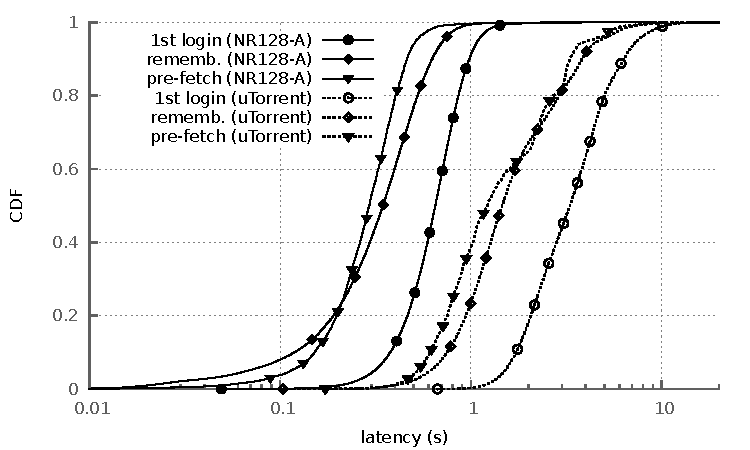
\includegraphics[width=.48\textwidth]{images/passwords-peer-to-peer/latencyCDF}
% 	\figlabel{latencyNr128aCDF}
% }
% \subfigure[$\mu$Torrent times]{
% 	\includegraphics[width=.48\textwidth]{images/passwords-peer-to-peer/latencyuTorrentCDF}
%   \figlabel{latencyuTorrentCDF}
% }
%   \caption{CDF for login latency in the three modes: First time login,
% remembered credentials, and first time login after password entry. Network
% operations assumed to have costs of BitTorrent mainline DHT lookup
% operations using NR128-A or $\mu$Torrent strategy~\cite{JimenezOK11}.} 
% \end{figure*}

\begin{figure}
 \centering
 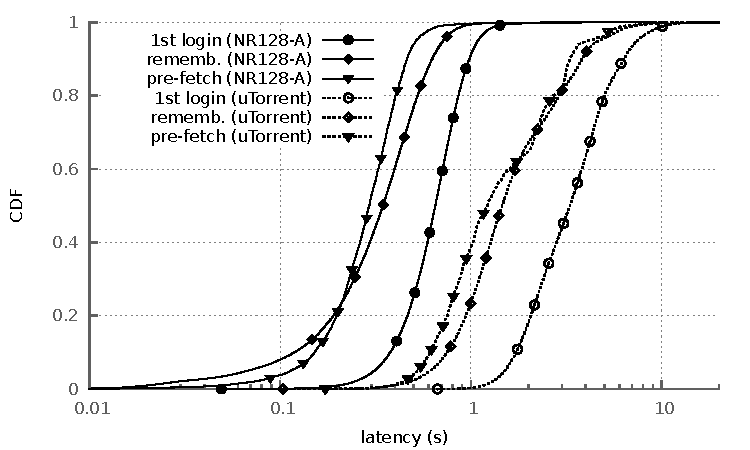
\includegraphics[width=.487\textwidth]{images/passwords-peer-to-peer/latencyCDF}
 \caption{CDF for login latency in three modes: First time login,
remembered logins, and first time login after password entry (pre-fetch). Network 
operations are assumed to have costs of BitTorrent mainline DHT lookups,
using NR128-A (solid lines) or $\mu$Torrent strategy (dashed lines)~\cite{JimenezOK11}.} 
 \figlabel{latencyCDF}
\end{figure}

We believe that the main performance-critical operation is logging
in~\cite{Rushinek86}. We believe that for all other operations,
latency on the order of a few seconds can be acceptable, and even a minute if they are run in the background. Thus, we only present results for logging in, but note
that as the operations for other protocols are similar, results are
expected to be similar. The performance cost of our protocols is
dominated by network operations. However, to slow down password
guessing attempts, one may wish to force the key derivation procedure
to be slow, to the point of making that cost dominant.

When evaluating the protocols, we parallelized network operations where
possible. Logging in for the first time and remembering the credentials for
future logins is then a sequence of two network operations, followed by key
derivation, followed by three parallel network operations. In a password
login, it is also possible to pre-fetch some of the information after the user
has entered her username, but before she enters her password. In
particular, as soon as the username is known, the filename $F_{LI}$ can be
retrieved from the DHT, and the file can be read. Decryption of the file and
further processing is then only possible after the user enters her password.
To evaluate % the gains of 
this speed-up, we computed the time it takes to
finish the login after the user has entered her password. The time to fetch
the two files is identical to the time to do a remembered login, and it is
sufficiently small that the data can realistically be retrieved while the user
is typing her password.

\begin{table}
\caption{Latencies of protocols, in milliseconds.}
\tablabel{latencies}
\centering
\newcommand{\mc}[3]{\multicolumn{#1}{#2}{#3}}
\begin{tabular}{lcccccc}
% 	\toprule
    & \mc{2}{c}{Network Op.~\cite{JimenezOK11}} & \mc{2}{c}{First Login} & \mc{2}{c}{Remem.\ Login}\\
	\cmidrule{2-7}
	DHT & median & $99^{\mathrm{th}}$  & median & $99^{\mathrm{th}}$  & median & $99^{\mathrm{th}}$  \\
	\midrule
	NR128-A & 164 & 567 & 650 & 1362 & 346 & 915 \\
	$\mu$Torrent & 647 & 5140 & 3299 & 10154 & 1456 & 7148 \\
	\bottomrule
\end{tabular}
\end{table}

To determine the sensitivity of our performance to implementation
characteristics, we evaluated our protocol for two different client strategies 
in the BitTorrent Mainline DHT:
The NR128-A algorithm~\cite{JimenezOK11}, and the
$\mu$Torrent client's implementation. We present these performance numbers in
\figref{latencyCDF} and 
\tabref{latencies}. Firstly, we observe that with a fast storage, our login
protocol is very fast, with a median login time of 650\,ms the first time, and
346\,ms for remembered logins. Comparing the results, we
observe that our protocols are indeed sensitive to storage latency. While
performance results building on $\mu$Torrent data are slightly above recommended
levels \cite{ToliaAS06}, we still consider them within range of acceptability
for P2P.

When evaluating these numbers, we assumed that the run-time of the KDF
function is negligible. As a system designer, one may wish to pick a slow KDF
(\eg bcrypt~\cite{DBLP:conf/usenix/ProvosM99}), as this slows down
password guessing attempts. Any latency intentionally added via the KDF would
affect the first-time login (after the password entry) times.


\subsection{Parameters for E-mail Password Recovery} \seclabel{evalemail}

%\begin{figure}
%  \centering
%	\includegraphics[width=.45\textwidth]{images/passwords-peer-to-peer/fixedn}
%  \caption{E-mail recovery: availability (probability of an immediately 
%successful password recovery) vs. security (success probability of an
%attacker, controlling 10\% or 25\% of the nodes) 
%for different $k$ ($n = 12$).}
%  \figlabel{fixedn}
%\end{figure}

%\begin{figure}
%  \centering
%	\includegraphics[width=.45\textwidth]{images/passwords-peer-to-peer/fixedk}
%  \caption{E-mail recovery: availability vs. security for different $n$ ($k$ = $n/2$)}
%  \figlabel{fixedk}
%\end{figure}

%\item Explain that there is a trade-off between three parameters (outlined
%below): availability, attacker success rate, and storage space
There are trade-offs between availability, security, and storage space in our e-mail based password recovery protocol.

%Describe the selection of $k$ parameter for a fixed $n$, a trade-off
%between availability and attacker success rate (\figref{fixedn})
For the selection of $k$, the minimum number of peers required to
recover the password, there is a direct trade-off between security and
availability.  Lower choices of $k$ increase the risk of an adversary,
controlling a significant number of nodes, to break into the user's
account. A higher $k$ reduces the availability of the recovery
functionality, which reflects the chances of a user to immediately
succeed with the password recovery.  However, if the user does not
instantly receive $k$ answers, she can simply wait until enough peers
are online.


We believe a reasonable choice of parameters is $n = 16$ and $k = n/2$. With
these numbers, using the availability data from Rzadca\etal~\cite{RzadcaDB10},
there is a 96\% probability of immediate recovery of a lost password. A very
strong attacker, corrupting 25\% of the nodes in the system, would still only
be able to access the user's account with probability 3\%.  The analysis of
parameter choice here is similar to any P2P system using secret sharing, and
we refer to e.g., Vu\etal \cite{Vu_Aberer_Buchegger_Datta_2009} for a more
in-depth discussion.

\subsection{Scalability}

The latency of our protocols will scale similarly to DHTs or other distributed
storage systems. The data we used for evaluation is based on measurements on
the largest deployed DHT, demonstrating that performance is good with
extremely large user numbers. Performance may in fact be worse for a small
system, as there are then fewer nodes, meaning that it is less likely to find
data at a nearby node. To bootstrap the system with good performance when it
is small, a very simple distributed storage using one or a few super-nodes
would be one approach. Storage requirements per user are also small, with a
few files per user and small file sizes. From this, we conclude that our
system is likely to scale well with the number of users.

\section{Conclusions and Future Work} \seclabel{conclusions}

The pros and cons of password-based authentication have been extensively
debated. We believe that for some applications, a username-password pair
provides an appropriate level of security. We argue that incorporating a
well-known authentication scheme may assist in user adoption of P2P systems
for more complex tasks than file sharing. To the best of our knowledge, ours
is the first work to focus on password-based logins in a P2P setting,
including mechanisms to recover a forgotten password. Our protocols are new
(but our security questions are similar to~\cite{FrykholmJ01}), relatively
straightforward, and we believe, they are an important first step towards
usable authentication in P2P. 

The performance of our mechanisms in terms of delay varies according
to the underlying DHT or P2P system in general and in relation to how
much intentional delay is added by parameterizing cryptographic
functions. Overall, however, our evaluation results show that for user
satisfaction~\cite{Rushinek86}, the delays can be kept at a very
acceptable level~\cite{ToliaAS06}.

While we have provided an initial discussion of the
security properties of our protocol here, future work will include a thorough
security analysis. Our scheme allows offline password guessing attacks, which
will also be addressed in future work.

\section*{Acknowledgments}

We thank Raúl Jiménez\etal{} %and his co-authors of
\cite{JimenezOK11} for sharing their measurement results and Jay Lorch for
excellent work as a shepherd of this paper. This research has been funded by
the Swedish Foundation for Strategic Research grant SSF FFL09-0086 and the
Swedish Research Council grant VR 2009-3793.


% last page column balancing (break column after specified bib entry)
%\IEEEtriggeratref{7}


% \bibliographystyle{IEEEtran}
% \bibliography{p2plogin}

% \end{document}